\let\negmpace\undefined
\let\negthickspace\undefined
\documentclass[journal]{IEEEtran}
\usepackage[a5paper, margin=10mm, onecolumn]{geometry}
%\usepackage{lmodern} % Ensure lmodern is loaded for pdflatex
\usepackage{tfrupee} % Include tfrupee package
\setlength{\headheight}{1cm} % Set the height of the header box
\setlength{\headsep}{0mm}     % Set the distance between the header box and the top of the text
\usepackage{gvv-book}
\usepackage{gvv}
\usepackage{cite}
\usepackage{amsmath,amssymb,amsfonts,amsthm}
\usepackage{algorithmic}
\usepackage{graphicx}
\usepackage{textcomp}
\usepackage{xcolor}
\usepackage{txfonts}
\usepackage{listings}
\usepackage{enumitem}
\usepackage{mathtools}
\usepackage{gensymb}
\usepackage{comment}
\usepackage[breaklinks=true]{hyperref}
\usepackage{tkz-euclide} 
\usepackage{listings}
% \usepackage{gvv}                                        
\def\inputGnumericTable{}                                 
\usepackage[latin1]{inputenc}                                
\usepackage{color}                                            
\usepackage{array}                                            
\usepackage{longtable}                                       
\usepackage{calc}                                             
\usepackage{multirow}                                         
\usepackage{hhline}                                           
\usepackage{ifthen}                                           
\usepackage{lscape}
\renewcommand{\thefigure}{\theenumi}
\renewcommand{\thetable}{\theenumi}
\setlength{\intextsep}{10pt} % Space between text and floats


\renewcommand{\thetable}{\theenumi}
\begin{document}
\bibliographystyle{IEEEtran}
\title{Question-9-9.2-33}
\author{EE24BTECH11035 - KOTHAPALLI AKHIL}
% \maketitle
% \newpage
% \bigskip
{\let\newpage\relax\maketitle}
\vspace{-10mm}
\textbf{Question}:\\
Find the area of the region enclosed by the parabola $x
^2 = y$ and the line $y = x + 2$.\\
\textbf{Solution}:\\
We will express both the parabola and the line equations in matrix form and use the given method to calculate the area between them.\\

The general conic form for a parabola $ax^2 + 2bxy + cy^2 + 2dx + 2ey + f = 0$ can be represented by matrices:
\begin{equation}
V = \begin{pmatrix} a & b \\ b & c \end{pmatrix}, \quad u = \begin{pmatrix} d \\ e \end{pmatrix}, \quad f
\end{equation}

For the parabola $x^2 = y$, the matrix representation becomes:
\begin{equation}
V_{\text{parabola}} = \begin{pmatrix} 1 & 0 \\ 0 & 0 \end{pmatrix}, \quad u_{\text{parabola}} = \begin{pmatrix} 0 \\ -\frac{1}{2} \end{pmatrix}, \quad f_{\text{parabola}} = 0
\end{equation}



The line equation $y = x + 2$ can also be expressed in matrix form as:
\begin{equation}
h^T x + m = 0
\end{equation}
Where $h$ is the vector of coefficients and $m$ is the constant.

For $y = x + 2$, we have:
\begin{equation}
h_{\text{line}} = \begin{pmatrix} 0 \\ 0 \end{pmatrix}, \quad m_{\text{line}} = \begin{pmatrix} 1 \\ 1 \end{pmatrix}
\end{equation}
To find the intersection points of the parabola $x^2 = y$ and the line $y = x + 2$, we substitute $y = x + 2$ into the parabola equation:
\begin{equation}
x^2 = x + 2
\end{equation}
\begin{equation}
x^2 - x - 2 = 0
\end{equation}
\begin{equation}
(x - 2)(x + 1) = 0
\end{equation}
Thus, $x = 2$ or $x = -1$.

Substitute these $x$-values back into the line equation to get the corresponding $y$-values:
\begin{align}
y(2) &= 2 + 2 = 4, \\
y(-1) &= -1 + 2 = 1
\end{align}
So, the points of intersection are $\myvec{-1\\1}$ and $\myvec{2\\4}$.\\
The area between the parabola and the line is given by the integral of the difference between the two curves.\\ The general form for calculating the area between two curves $y_1$ and $y_2$ from $x_1$ to $x_2$ is:
\begin{equation}
Area = \int_{x_1}^{x_2} (y_1 - y_2) \, dx
\end{equation}
Here, $y_1 = x + 2$ and $y_2 = x^2$.

Thus, the area is:
\begin{equation}
\text{Area} = \int_{-1}^{2} \left( (x + 2) - x^2 \right) \, dx
\end{equation}
\begin{equation}
\int_{-1}^{2} \left( x + 2 - x^2 \right) \, dx = \left[ \frac{x^2}{2} + 2x - \frac{x^3}{3} \right]_{-1}^{2}
\end{equation}
Substitute the limits:
\begin{equation}
= \left[ \frac{2^2}{2} + 2(2) - \frac{2^3}{3} \right] - \left[ \frac{(-1)^2}{2} + 2(-1) - \frac{(-1)^3}{3} \right]
\end{equation}
\begin{equation}
= \left[ \frac{4}{2} + 4 - \frac{8}{3} \right] - \left[ \frac{1}{2} - 2 + \frac{1}{3} \right]
\end{equation}
\begin{equation}
= \left[ 2 + 4 - \frac{8}{3} \right] - \left[ \frac{1}{2} - 2 + \frac{1}{3} \right]
\end{equation}
\begin{equation}
= \left( 6 - \frac{8}{3} \right) - \left( -\frac{3}{2} + \frac{1}{3} \right)
\end{equation}
\begin{equation}
= \frac{10}{3} + \frac{11}{6} = \frac{60 + 22}{18} = \frac{82}{18} = \frac{41}{9}
\end{equation}

Thus, the area of the region enclosed by the parabola and the line is $\frac{41}{9}$ square units.
\begin{figure}[h!]
	\centering
	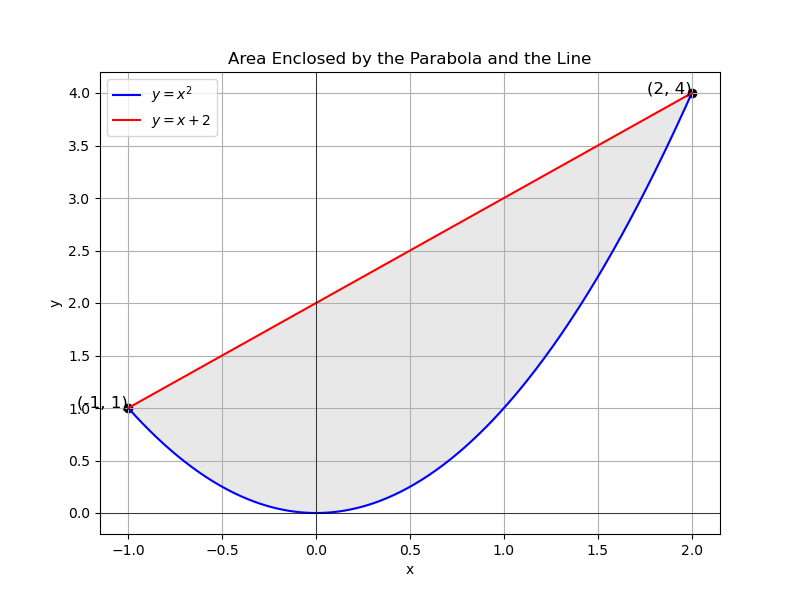
\includegraphics[width=0.5\linewidth]{figs/Figure_1.png}
	\caption{Area enclosed between parabola and Line}
	\label{stemplot}
\end{figure}	

\end{document}
